\documentclass[12pt]{article}

\usepackage[total={6.5in,8.75in}, top=2.4cm, left=2.4cm]{geometry}
\usepackage{lineno}
\usepackage{amsmath}
%\usepackage{amssymb}    % used for symbols in figure legends
\usepackage{graphicx}
\usepackage[round,colon,authoryear]{natbib}

\usepackage{bm}
\usepackage{float}
\usepackage{amsmath}
\usepackage{amsfonts}
\usepackage{hyperref}
\usepackage{verbatim}
\usepackage{soul}
\usepackage{color}


\bibliographystyle{../asa} % kluwer, plos-natbib, pnas-natbib


\title{Ecological Distance in Spatial Capture-Recapture Models}

\author{
{\bf J. Andrew Royle}\\ 
USGS Patuxent Wildlife Research Center, Laurel MD \\ \\
{\bf Richard B. Chandler} \\ 
USGS Patuxent Wildlife Research Center, Laurel MD\\ \\
{\bf Kimberly Gazenski} \\
USGS Patuxent Wildlife Research Center, Laurel MD\\ \\
{\bf Tabitha A. Graves} \\
Northern Arizona University, Flagstaff AZ \\ \\
}



\begin{document}
%\begin{spacing}{1.9}

\maketitle

\date

\newpage

\linenumbers

\begin{flushleft}
{\em \bf Abstract}


\end{flushleft}

\section{Introduction}


%% this material is a general introduction for a manuscript
Spatial capture-recapture models are a relatively new class of models
for estimating animal density from capture-recapture data with
auxiliary information about individual capture locations
\citep{borchers_efford:2008, royle_young:2008, efford_etal:2009, royle_etal:2009}.  The basic idea is to express encounter probability of
individuals as a function of the distance between individual center of
activity, say ${\bf s}_{i}$, and trap location, say ${\bf x}_{j}$.  In
these models ${\bf s}_{i}$ is regarded as a latent variable and
conventional methods of statistical inference either based on marginal
likelihood \citep{borchers_efford:2008} or Bayesian analysis by MCMC
\citep{royle_young:2008}.

While the models are a relatively recent innovation, their use is
already becoming widespread \citep{efford_etal:2009,
  gardner_etal:2010, kery_etal:2010, efford:2011UO,
  gopalaswamy_etal:2012, foster_harmsen:2012} because they resolve critical problems with using
ordinary non-spatial capture-recapture methods such as ill-defined
area sampled, heterogeneity in encounter probability due to the
juxtaposition of individuals with traps, and they provide a framework
for modeling of trap-specific covariates.  Furthermore, essentially
all real capture-recapture studies produce auxiliary spatial
information and therefore SCR models are directly relevant to standard
data collected from such studies. Indeed, the use of ordinary
capture-recapture models essentially admits a model misspecification
(i.e. homogeneous encounter probability) by ignoring the explicit
spatial information.

Every application of SCR models so far has been based on encounter
probability models in which distance between individual activity
center and trap location is defined by a function of simple Euclidean
distance.  While these will often be sufficient for practical
purposes, especially in small data sets, sometimes developing more
complex models of the detection process as it relates to space usage
of individuals will be useful.  Animals may not judge distance in
terms of Euclidean distance but, rather, according to quality of local
habitat, landscape connectivity, perceived mortality risk, and other
considerations that statisticians might not really
understand. Moreover, because encounter probability and the distance
metric upon which that is based represent outcomes of individual
movements about their home range, ecologists might have explicit
hypotheses about how environmental variables affect the distance
metric, and it is therefore desireable to incorporate these hypotheses
directly into SCR models so that they may be formally evaluated
statistically.
As an example of the potential problem of parameterizing SCR models
using Euclidean distance, imagine a study area bisected by a large
semi-permeable barrier. In traditional SCR models, the probability of
capturing an animal in a trap located on the opposite side of the
barrier would simply be a function of distance, whereas in reality it
should be a function of both distance and the permeability of the
barrier. Such situations are extremely common in capture-recapture
studies where multiple habitats occur in the study area or when
animals use linear features such as trails, corridors, or rivers.

In this paper we develop models for encounter probability based on
alternative distance metrics that account for ecological
considerations -- which, in keeping with the conventions in the
ecological literature, we will call ``ecological distance''. In
particular, we adopt a cost-weighted distance metric (the least-cost path) 
used widely in landscape ecology for modeling connectivity,
movement and gene flow
\citep{adriaensen_etal:2003,manel_etal:2003,mcrae_etal:2008}. In the
context of SCR models we can use this as the basis for computing the
distance between traps and individuals activity centers. In this way
we can explicitly accommodate landscape structure and 
account for how animals use space in SCR models. We develop a
likelihood-based inference framework for SCR model parameters using
this new distance metric when the ecological distance function is
known.  We show that the MLEs are approximately unbiased in moderate
sample sizes, as expected, but also that the misspecified model based
on Euclidean distance can produce substantial bias in estimates of $N$
and hence density.  Finally, we extend the model to allow for the case
where the distance metric is only known by a covariate and the
relative ``cost'' is estimated by maximum likelihood in addition to
other encounter probability parameters and density.


\section{Spatial Capture-Recapture}

A number of distinct observation models have been proposed for
spatial-capture situations, including Poisson, multinomial or binomial
observation models. Here we focus on the binomial model in which we
suppose that $J$ traps at locations ${\bf x}_{j}$ are operated for $K$
periods (e.g., nights) although our development of cost-distance
models is directly applicable to other observation models without any
further technical considerations. The binomial model is most directly
relevant to devices such as ``hair snares''
\citep{woods_etal:1999,gardner_etal:2010} or scent sticks
\citep{kery_etal:2010} for which individuals can only be encountered a
single time per observation occasion.

The observations are the individual- and trap specific counts $y_{ij}$
which are binomial counts with sample size $K$ and probabilities
$p_{ij}$. A standard encounter probability model
\citep{borchers_efford:2008} is the Gaussian model in which
\begin{equation}
log(p_{ij})= \theta_{0} + \theta_{1} dist({\bf x}_{j} - {\bf s}_{i})^{2}
\label{eq.encounter}
\end{equation}
or, equivalently, 
\[
p_{ij} = \lambda_{0} exp(-  dist({\bf x}_{j} - {\bf s}_{i})^{2}
/(2\sigma^{2}) )
\]
where $\theta_{0} = log(\lambda_{0})$ and $\theta_{1} =
-1/(2\sigma^2)$. 

In all previous applications of SCR models the normal Euclidean
distance has been used, i.e., $ dist({\bf x}_{j} - {\bf s}_{i}) =
||{\bf x}_{j} - {\bf s}_{i}||$, and the parameters $\theta_0$ and
$\theta_1$ have been estimated using standard methods (likelihood or
Bayesian). These methods regard ${\bf s}_{i}$ as realizations of a
point process (i.e., latent variables) and remove them from the
likelihood either under a model of ``uniformity'' in which ${\bf s}
\sim \mbox{Uniform}({\cal S})$ where ${\cal S}$ is the state-space of
the point process, or in which covariates might affect the spatial
distribution of individuals (..... XYZ .....). Alternative detection
models are commonly used, but they are all functions of Euclidean
distance and so we do not them here.

The critical consideration that motivates our work is that 
 Euclidean distance metric is unaffected by habitat or landscape
structure, and it implies that space usage of individuals is
stationary, isotropic and symmetric which may be unreasonable in most
applications.  For example, if the common detection model based on a
bivariate
normal probability distribution function is used, then the implied
space
usage by {\it all} individuals, no matter their location in space or
local habitat conditions, is symmetric with circular contours of 
usage intensity (density contours of the pdf). 
Subsequently we provide an extension of this class of SCR models that
accommodates alternative distance metrics that explicitly incorporate
information about the landscape so that a unit of distance is variable
depending on identified covariates. Thus, ``where'' an individual
lives on the landscape, and the state of the surrounding landscape,
will determine the character of its usage of space. In particular, we
suggest distance metrics that imply irregular, asymmetric and
non-stationary home ranges of individuals (e.g., see Figure XYZ
described
below).


\section{Cost Distance}

We use a cost-weighted distance metric in the package \mbox{\tt
gdistance} \index{R package!gdistance} which computes the distance 
between points by accumulating pixel-specific costs assigned by the user 
(but we consider estimating these in Sec. XYZ). The idea is widely used in
landscape ecology for modeling connectivity, movement and gene flow
\citep{adriaensen_etal:2003}. As is customary for reasons of
computational tractability we consider a discrete landscape defined by a 
raster of some prescribed resolution. The distance between any two points 
${\bf x}$ and ${\bf x}'$ can be represented by a sequence of line segments 
connecting a sequence of neighboring  pixels say 
${\bf l}_{1},{\bf l}_{2},\ldots,{\bf l}_{m}$. Then the cost-weighted distance 
between ${\bf x}$ and ${\bf x}'$ is
\begin{equation}
 d({\bf x},{\bf x}')
  =  \sum_{i=1}^{m-1} cost({\bf l}_{i},{\bf l}_{i+1})||{\bf l}_{i} - {\bf l}_{i+1}||
\label{eq.costweighted}
\end{equation}
where $cost({\bf l}_{i},{\bf l}_{i+1})$ is the user-defined cost function
to move 
from pixel ${\bf l}_{i}$ to neighboring pixel ${\bf l}_{i}$ in the sequence.
In this paper we consider modeling cost as a function of covariates
defined on every pixel of the raster according to, for example using a
single
covariate $z(x)$:
\begin{equation}
 log(cost(x))=  \theta_{2} z(x) 
\label{eq.cost}
\end{equation}
Thus, if $\theta_{2} = 0$ then substituting $cost(x)$ into
Eq. \ref{eq.costweighted} will produce the ordinary Euclidean distance
between points. 
In practical applications, variables that
influence the cost of moving across the landscape include things like
highways (e.g. \citet{epps_etal:2005}), elevation
(e.g.\citet{cushman_etal:2006} Cushman et al. 2006), 
ruggedness (e.g. \citet{epps_etal:2007}), snow cover (e.g.\citet{schwartz_etal:2009}), 
distance to escape terrain (e.g. \citet{shirk_etal:2010}), or predator density 
(CITE elk/wolf paper).  Together multiple environmental variables create 
a resistance surface, which forms the linchpin of all connectivity 
planning \citep{spear_etal:2010}. 
.

Given the ``cost'' of each pixel, it is a simple matter to compute the
cost-weighted distance between any two pixels, along {\it any} path,
simply by accumulating the intermittent costs weighted by distances. 
To be consistent with our use of the {\bf R} package \mbox{\tt
  costDistance} \citep{vanetten:2011},
the incremental cost of moving from one pixel to another is the
distance-weighting of the {\it average} of the 2 pixel costs (see below).
In the context of spatial capture-recapture models (and, more
generally, landscape connectivity) we are concerned with the {\it
  minimum} cost-weighted distance between any two points.  That is, we
seek to find the 
sequence ${\bf l}_{1},{\bf l}_{2},\ldots,{\bf l}_{m}$ that minimizes
the objective function defined by Eq. \ref{eq.costweighted}.
This is done in some GIS packages and also in the {\bf R} package
\mbox{\tt costDistance} using the implementation of Dijkstra's algorithm \citep{dijkstra:1959}
found in the \mbox{\tt igraph} package \citep{csardi:2010}.

To formalize the use of cost-weighted distance in SCR models, we
substitute Eq. \ref{eq.costweighted} in the expression for encounter
probability (Eq. \ref{eq.encounter}) and maximize the resulting
likelihood (see the next section).

\subsection{Example of Computing Cost-weighted distance}

As an example of the cost-weighted distance calculation consider the
following landscape comprised of 16 pixels with unit spacing 
identified as follows, along with the pixel-specific cost:
\begin{verbatim}
  pixel ID                 Cost
  1  5  9  13          100   1   1  1
  2  6 10  14          100 100   1  1
  3  7 11  15          100 100 100  1
  4  8 12  16          100 100   1  1 
\end{verbatim}
Then we assign low cost of 1 to ``good habitat'' pixels (or pixels we
think of as ``highly connected'' by virtue of being in good habitat)
and, conversely, we assign high cost (100) to ``bad habitat''. So the
shortest cost-weighted distance between pixels 5 and 9 in this example
is just 1 unit, the shortest cost-distance between pixels 5 and 10 is
sqrt(2) units= 1.414214, the shortest distance between pixels 4 and 8 is 100
units, while the shortest cost-distance between 4 and 12 is 150.5. A
tough one is: what is the shortest distance between 7 and 16? A guy at pixel
7 can move diagonal and pay  $sqrt(2)*(100+1)/2 + 1 =72.41778$.

\begin{verbatim}
r<-raster(nrows=4,ncols=4)
projection(r)<- "+proj=utm +zone=12 +datum=WGS84"
extent(r)<-c(.5,4.5,.5,4.5)
costs1<- c(100,100,100,100,1,100,100,100,1,1,100,1,1,1,1,1)
values(r)<-matrix(costs1,4,4,byrow=FALSE)
par(mfrow=c(1,1))
plot(r,useRaster=F)
\end{verbatim}
The raster, in image form, is shown in Fig. \ref{ecoldist.fig.raster}.

\begin{figure}
\begin{center}
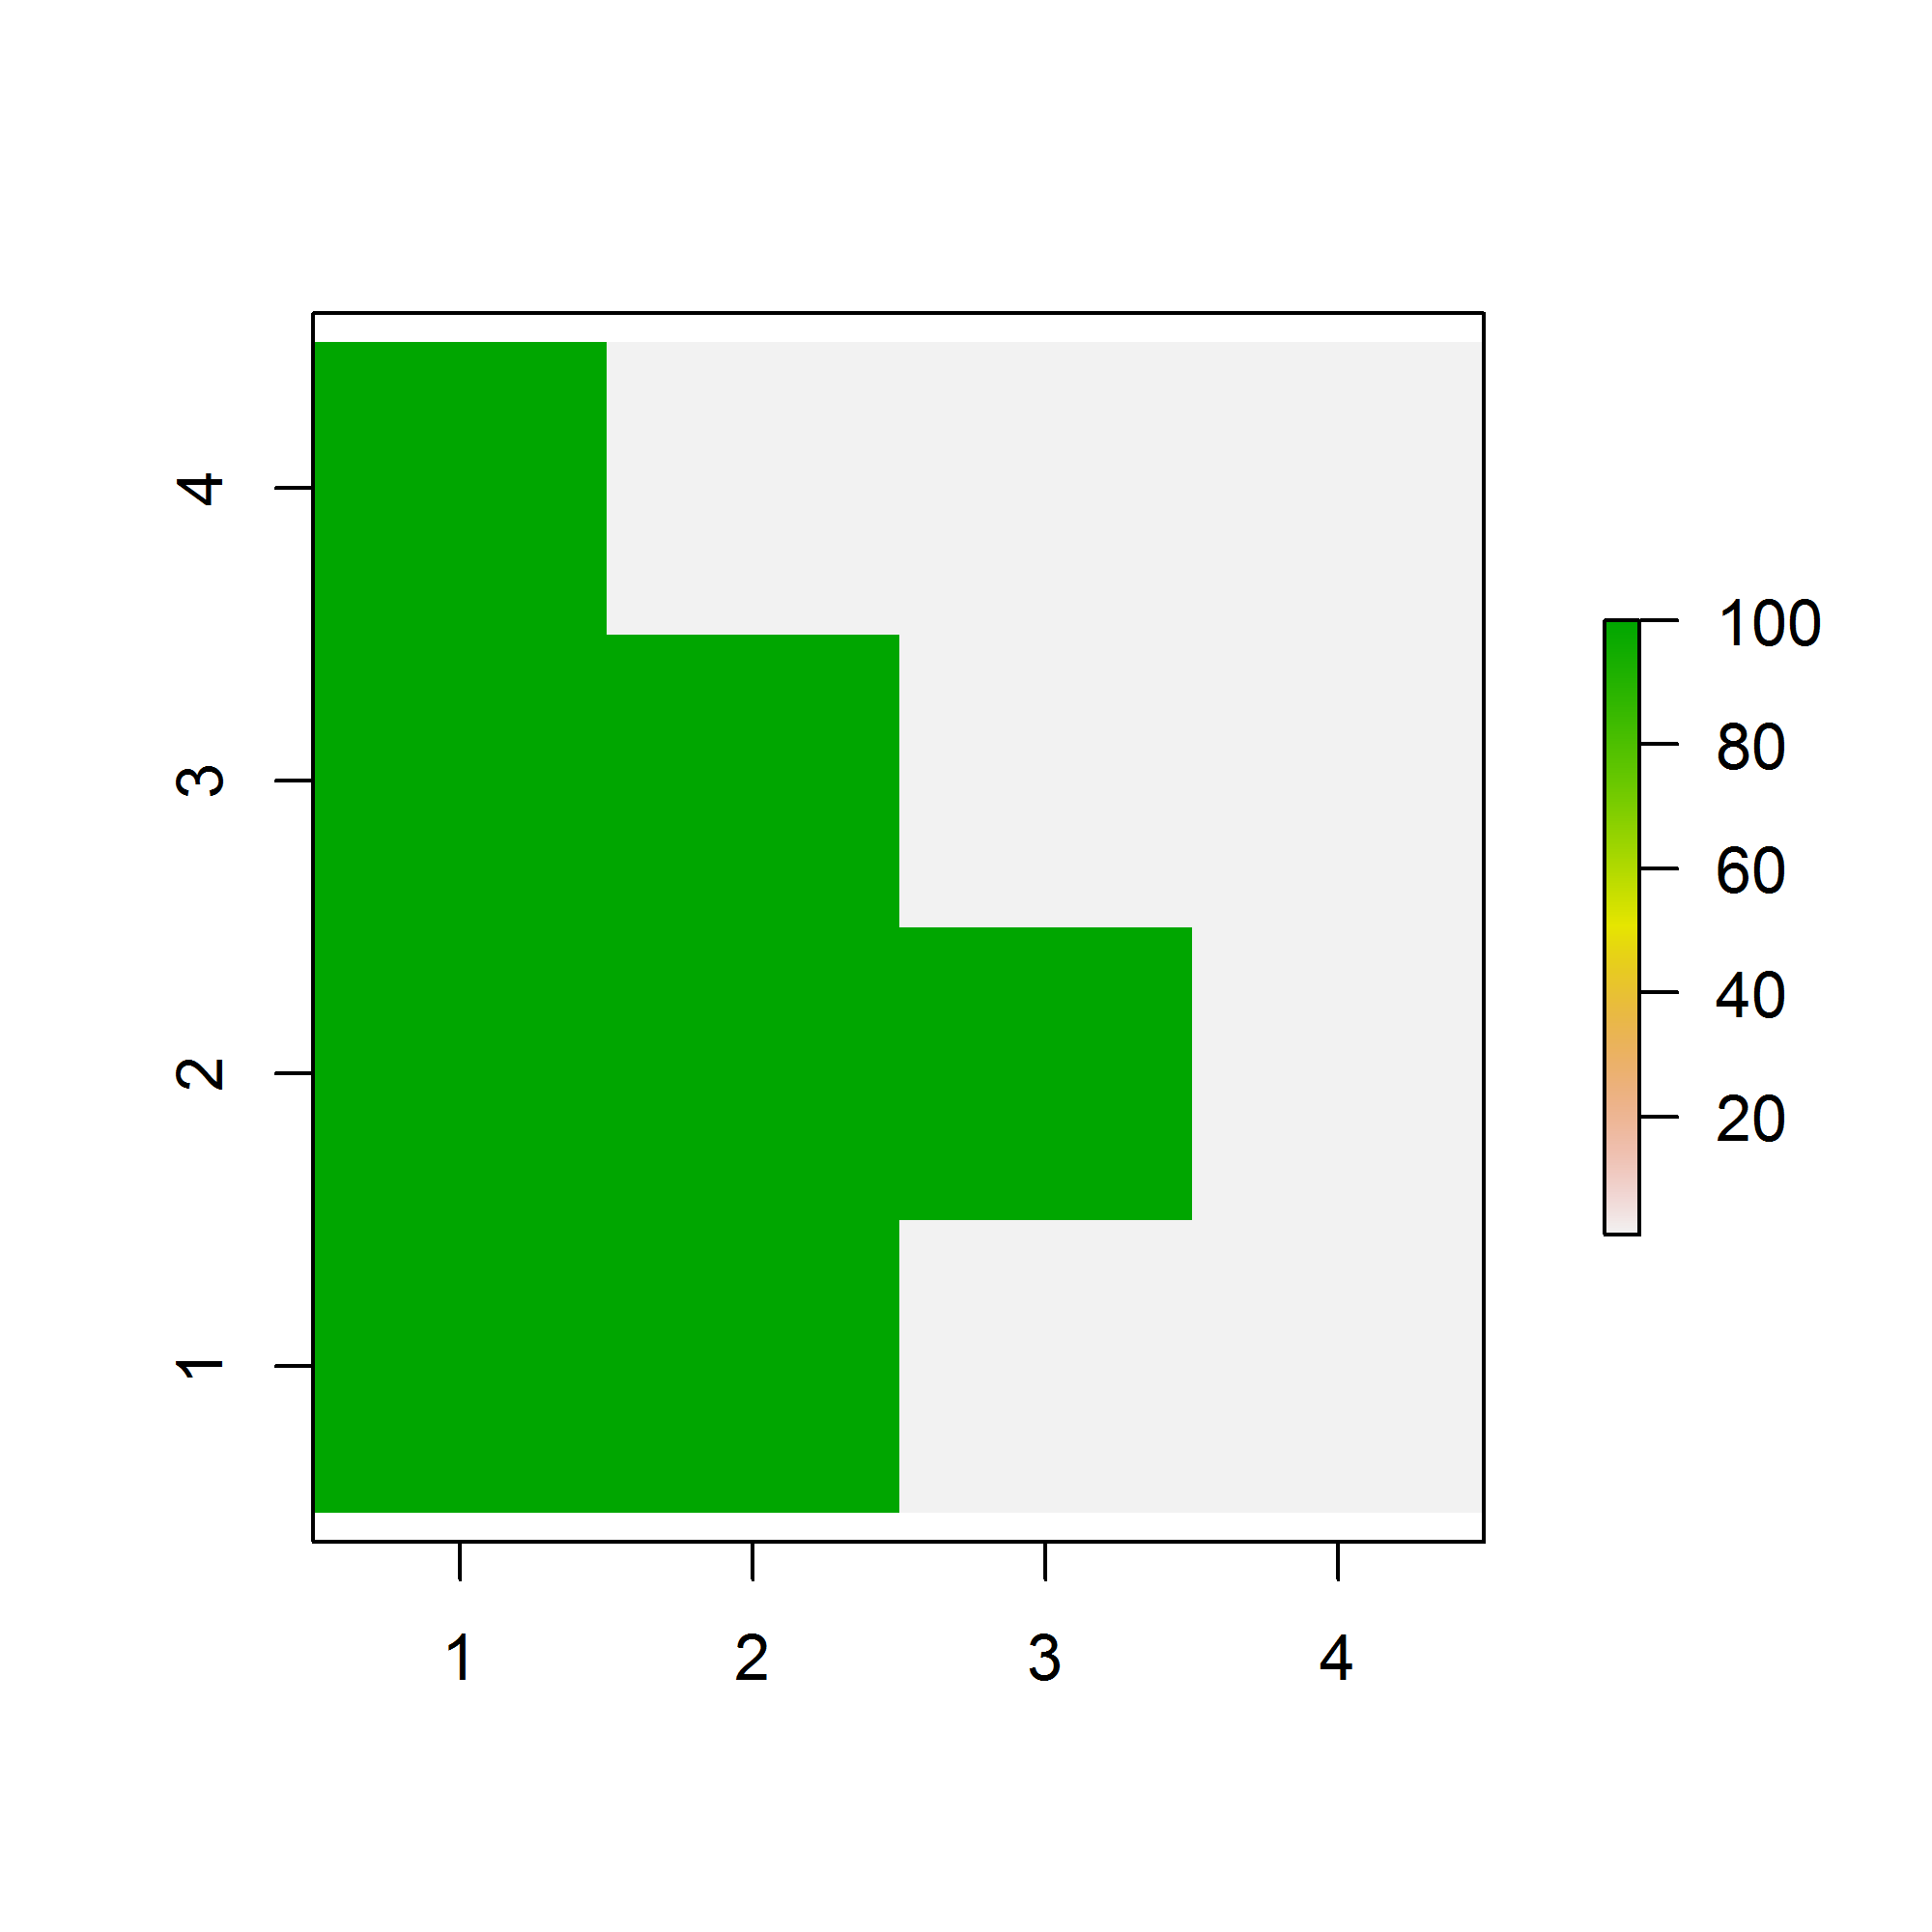
\includegraphics[height=3.25in,width=3.25in]{figs/raster_2values}
\end{center}
\caption{a 16 pt raster}
\label{ecoldist.fig.raster}
\end{figure}

Then we use the functions \mbox{\tt transition}, which calculates the cost of
moving between neighboring pixels, \mbox{\tt
  geoCorrection}  which modifies the costs of moving diagonally by the additional distance,
   and \mbox{\tt costDistance} to compute the distance
matrix. We define a set of points,
the center points of each raster, to compute the pair-wise cost-distances between all raster pixels.
 The commands altogether are as follows:
{\bf Tabitha}: Can you say something here about why this is 1/mean(x)?
\begin{verbatim}
#The transition function specifies that we'd like to use the mean of 
# 2 neighboring pixels as the weight and then takes the inverse to convert 
# the costs into conductances, which algorithms within gdistance and 
# igraph require. We use the argument directions= 8 to specify that 
# all 8 touching pixels are neighbors.)

tr1<-transition(r,transitionFunction=function(x) 1/mean(x),directions=8)
tr1CorrC<-geoCorrection(tr1,type="c",multpl=FALSE,scl=FALSE)
pts<-cbind( sort(rep(1:4,4)),rep(4:1,4))
costs1<-costDistance(tr1CorrC,pts)
outD<-as.matrix(costs1)
\end{verbatim}
Now we can look at the result and see if it makes sense to us. Here we
print the first 4 columns of this distance matrix and illustration a
couple of examples of calculating the minimum cost-weighted distance
between points:

\begin{verbatim}
These seem to check out for the most part but look at [4,1] -- this isn't right!

> outD[1:5,1:5]
         1         2        3        4         5
1   0.0000 100.00000 200.0000 205.2426  50.50000
2 100.0000   0.00000 100.0000 200.0000  71.41778
3 200.0000 100.00000   0.0000 100.0000 171.41778
4 205.2426 200.00000 100.0000   0.0000 154.74264
5  50.5000  71.41778 171.4178 154.7426   0.00000

\end{verbatim}


\subsection{Non-stationarity of home range structure}

When distance is defined by the cost-weighted distrance metric
given by Eq. \ref{eq.costweighted} then individual space-usage varies
spatially in response to the landscape covariate(s) used in the
distance metric. For example, using one of the covariates we use in
our simulation study below (Fig. \ref{ecoldist.fig.raster100}, right
panel)
with a Gaussian pdf detection function but having distance metric
defined
by Eq. \ref{eq.costweighted}, produces home ranges such as those shown
in Fig. \ref{fig.homeranges}.

\begin{figure}
\begin{center}
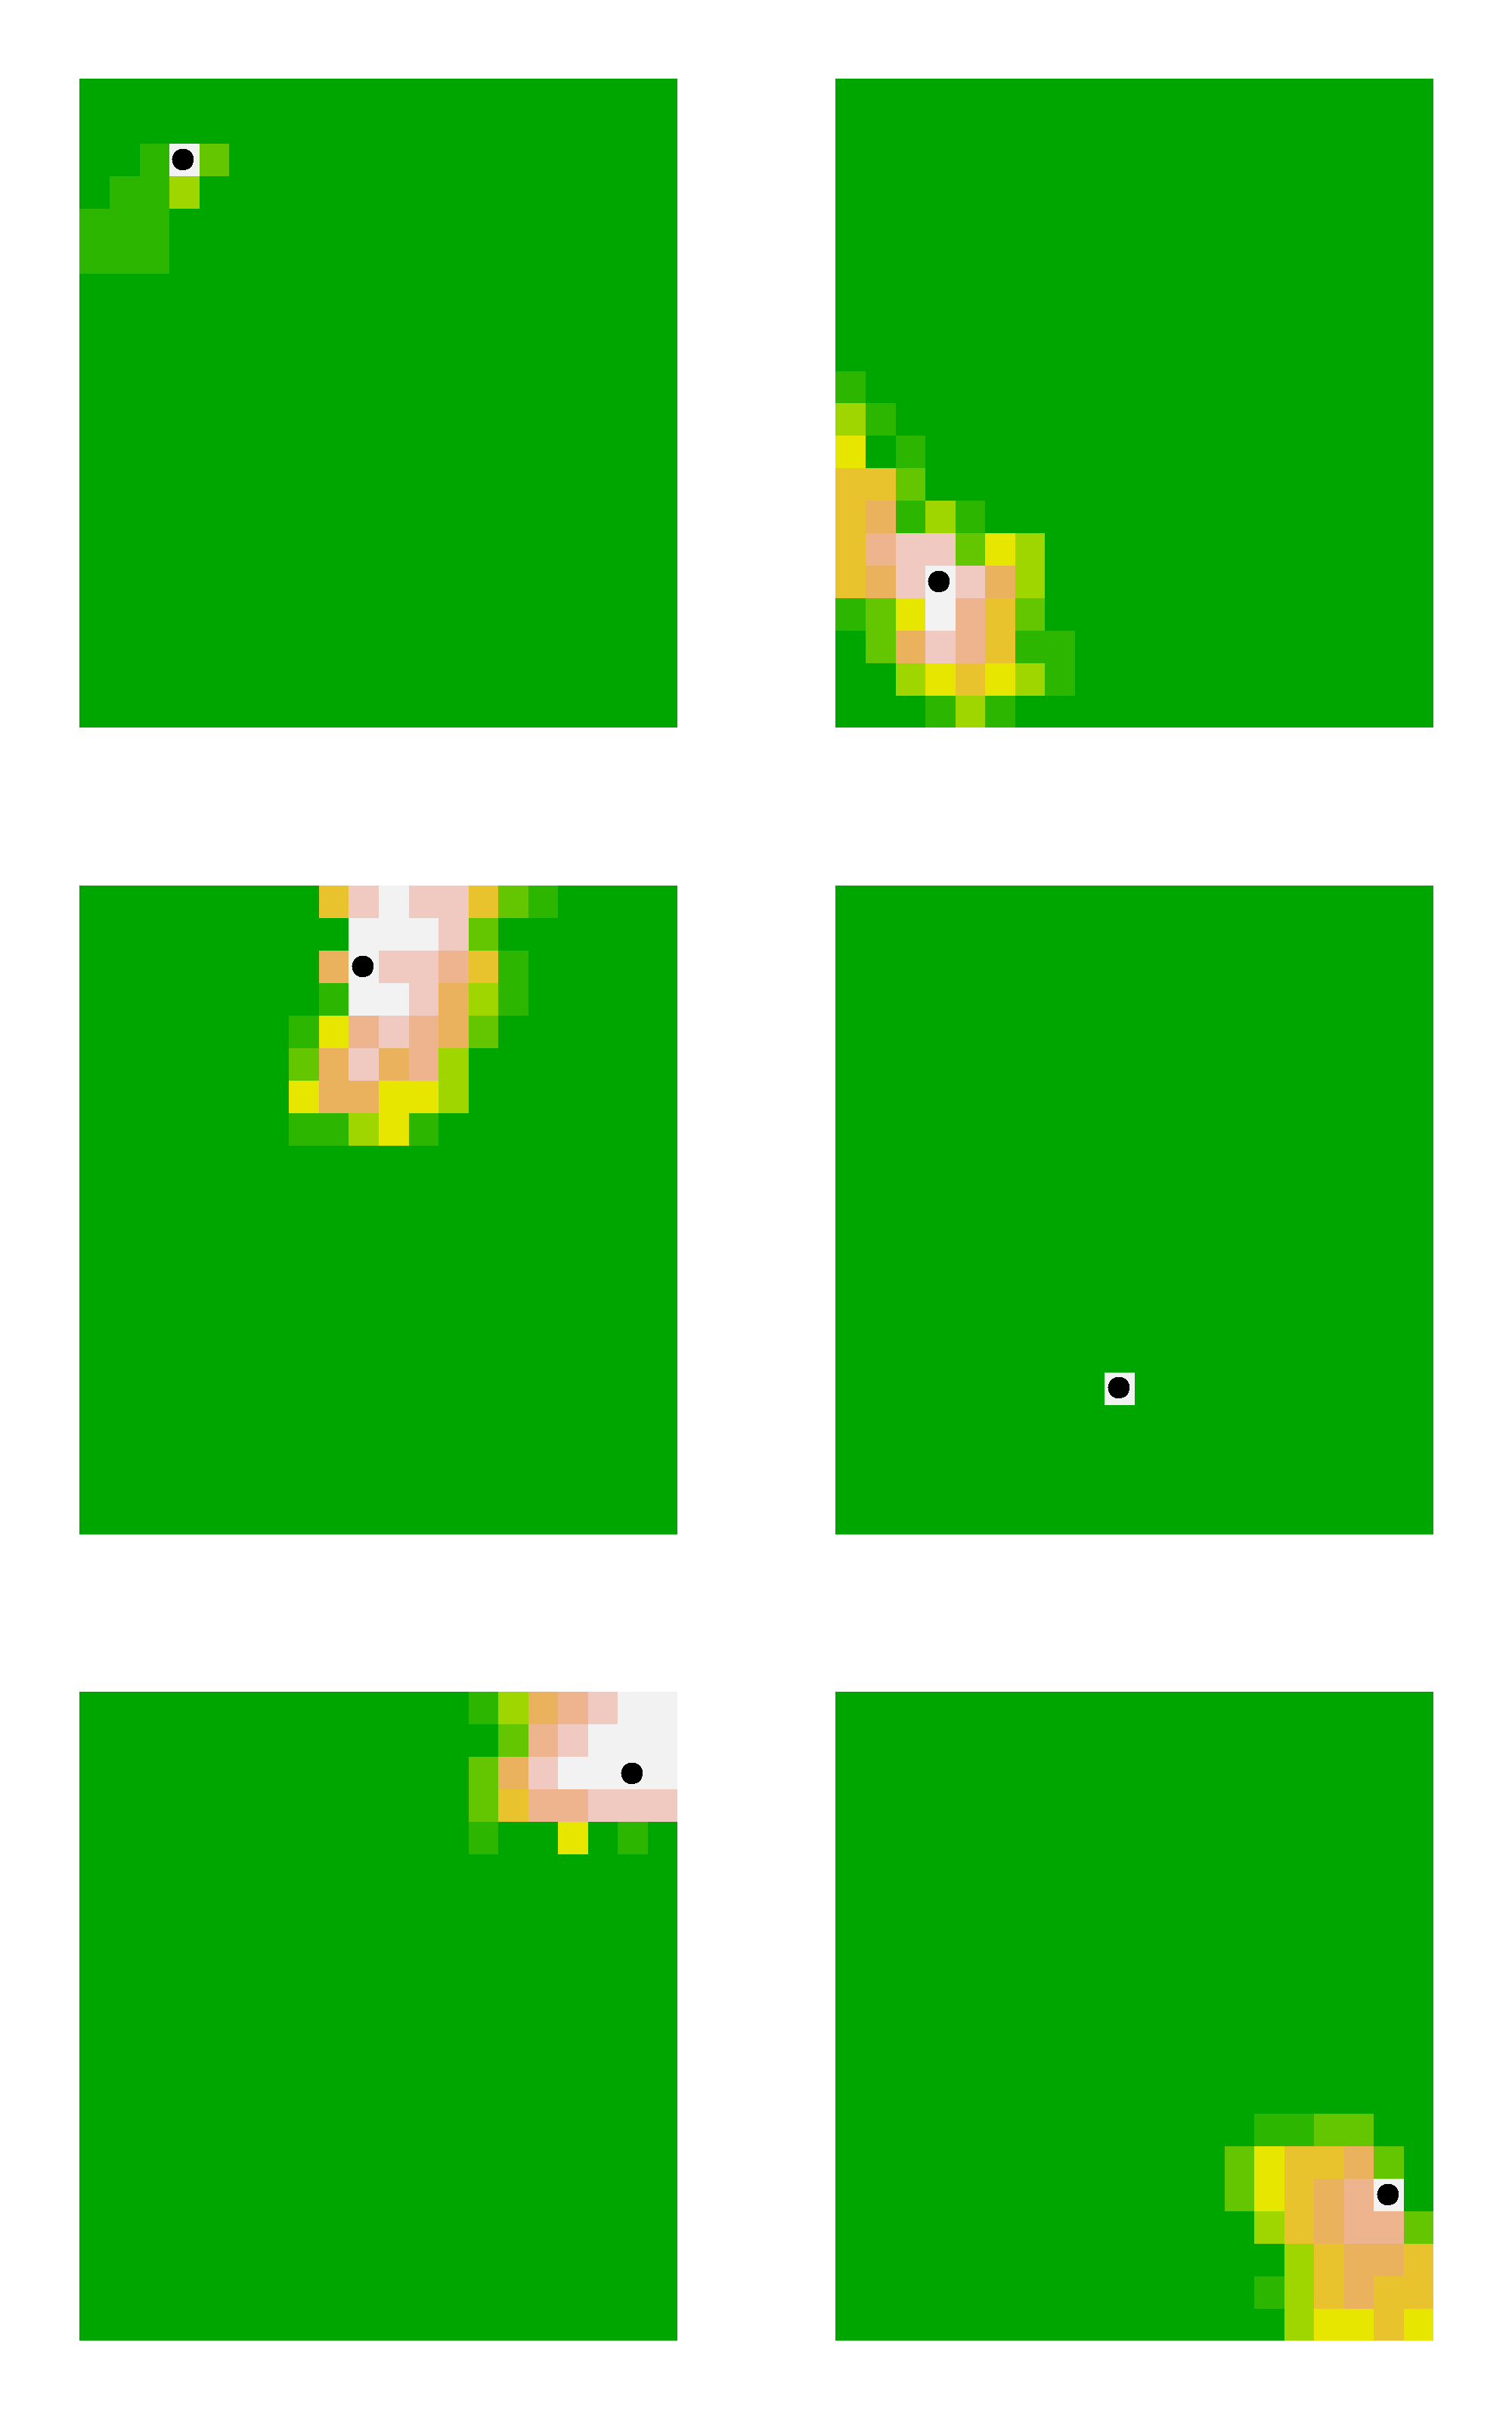
\includegraphics[height=6,width=3.75in]{figs/home_ranges}
\end{center}
\caption{6 typical home ranges}
\label{fig.homeranges}
\end{figure}



\section{Maximum likelihood estimation}

Here we develop a standard method of parameter estimation based on
the marginal likelihood. That is, the likelihood in which the latent
variables ${\bf s}$ are removed by integration \citep{borchers_efford:2008}. 

The individual- and trap-specific observations have a binomial
distribution conditional on the latent variable ${\bf s}_{i}$:
\begin{equation}
	y_{ij}| {\bf s}_{i} \sim \mbox{Bin}(K, p_{\theta}({\bf x}_{j},{\bf s}_{i}))
\label{mle.eq.cond-on-s}
\end{equation}
where we have indicated the dependence of $p_{ij}$ on ${\bf s}$ and
the vector of parameters ${\bm \theta}$ explicitly. The parameters
${\bm \theta}$ include whatever parameters are involved in the
cost-weighted distance function, i.e., at least $\theta_{2}$ from 
Eq. \ref{eq.cost}.
For the random effect we have ${\bf s}_{i} \sim  \mbox{Unif}({\cal
  S})$.
The joint distribution of the data for individual $i$ is the product
of $J$ binomial terms (i.e., contributions from each of $J$ traps):
\[
  [{\bf y}_{i} | {\bf s}_{i} , \theta] = 
  \prod_{j=1}^{J} \mbox{Bin}(K, p_{\theta}({\bf x}_{j},{\bf s}_{i}) )
\]
This assumes that encounter of individual $i$ in each
trap is independent of encounter in every other trap. Conditional on
${\bf s}_{i}$ this is reasonable in most applications in our view.
 The so-called marginal likelihood is computed by removing
${\bf s}_{i}$, by integration,  from the conditional-on-${\bf s}$
likelihood and regarding the {\it marginal} distribution of the data
as the likelihood. That
is, we compute:
\[
  [y|{\bm \theta}] = 
\int_{{\cal S}}  [ {\bf y}_{i} |{\bf s}_{i},{\bm \theta}] g({\bf s}_{i}) d{\bf s}_{i}
\]
where, under the uniformity assumption, we have
$g({\bf s}) = 1/||{\cal S}||$.
The joint likelihood for all $N$ individuals, assuming independence of
encounters among individuals, is the product of $N$ such terms:
\[
{\cal L}({\bm \theta} | {\bf y}_{1},{\bf y}_{2},\ldots, {\bf y}_{N}) = \prod_{i=1}^{N}
[{\bf y}_{i}|{\bm \theta}]
\]

The key operation for computing the likelihood is solving the
2-dimensional integration problem to remove ${\bf s}$. There are some
general purpose {\bf R} packages that implement a number of
multi-dimensional integration routines including \mbox{\tt adapt}
\citep{genz_etal:2007} and \mbox{\tt R2cuba} \citep{hahn_etal:2011}.
We won't rely on these extraneous {\bf R} packages but instead will
use perhaps less efficient methods in which we replace the integral
with a summation over an equal area mesh of points on the state-space
${\cal S}$ and explicitly evaluate the integrand at each point. We
invoke the rectangular rule for integration here in which the
integrand is evaluated on a regular grid of points of equal area and
then averaged.  Let $u=1,2,\ldots,nG$ index a grid of $nG$ points,
${\bf s}_{u}$, where the area of grid cell $u$ is constant.  In this
case, the integrand, i.e., the marginal pmf of ${\bf y}_{i}$, is
approximated by
\begin{equation}
         [{\bf y}_{i}|\theta] = \frac{1}{nG} \sum_{u=1}^{nG}  [ {\bf
            y}_{i} |{\bf s}_u, \theta]
\label{mle.eq.intlik}
\end{equation}

To deal with the fact that $N$ is unknown, 
there are two key issues that need to be addressed.
First is that 
we don't observe the all-zero encounter history so we have to
make sure we compute the probability for that ``all zero'' encounter history which
we do operationally by tacking a row of zeros onto the encounter history matrix. In
addition, we include the number of such all-zero encounter histories
as an unknown parameter of the model. Call that unknown quantity $n_{0}$.
In addition, we have to be sure to include a combinatorial term to
account for the fact that of the $n$ observed individuals there are
${N \choose n}$
 ways to realize a sample of size $n$. The combinatorial term
involves the unknown $n_{0}$ and thus it must be included in the likelihood.

To compute the integral requires that the bounds of integration are
specified, which is equivalent to prescribing the state-space of the
underlying point process, i.e., ${\cal S}$. Therefore density is
computed as $D({\cal S}) = N/||{\cal S}||$. In our simulation study
below we report $N$ as the two are equivalent summaries of the data
set once the state-space is fixed. 

We wrote an R function to evaluate the likelihood which we optimize
using the R function \mbox{\tt nlm}.
The R code is given as a script in the Appendix and the R package scr
is available on the website XYZ along with functions for simulating
data.


\section{Examples of Computing Cost-Distance}

In this section we provide an example that we think is typical of 
how cost-weighted distance models can be used in real
capture-recapture problems.
\begin{comment}
In particular, we will typically have a polygon coverage either in the
form of a GIS shapefile or a matrix of points or some other specific
format, and we want to put that polygon on a map and use the polygon
boundary in some way to generate pixel-specific costs. So we want to
see if points or raster pixels are in the polygon, or not, or how far
they are from the polygon boundary (cost might be related to distance)
and similar operations. In the following examples, we confront how to
do some of these operations in {\bf R}. 
\end{comment}

We define a $20 \times 20$ pixel raster with
extent $[0.5, 4.5] \times [0.5, 4.5]$.
We regard for the purposes of this example as a coarse landscape 
covariate, with (scaled) pixels having ,  say, a $2 \times 2$ km resolution. Thus, the raster
therefore
defines a landscape of $40 \times 40$ km and we suppose that 16 camera
traps are established at the integer coordinates (1,1), (1,2),
... (4,4). 
Maybe we are studying a population of ocelots or lynx or some other
spotted cat.
We suppose 
that each raster is characterized by a single covariate and we consider two specific
cases. First is an increasing trend from 
the NW to the SE, where $z(x)$ is defined as $z(x) = r(x) + c(x)$ where $r(x)$ and $c(x)$ are 
just the row and column, respectively, of the raster. 
This might define something related to distance
from an urban area or a gradient in habitat quality due to land use,
or environmental conditions. 
In the second case we make up a covariate by generating a field of spatially correlated
noise to emulate a typical patchy habitat covariate. The two covariates are shown in 
Figure XYZ. 

We define 
\[
 log(cost(x))=  \beta z(x) 
 \]
where $\beta = 1$ which we regard as known. With $\beta=0$ then the model reduces to
one in which the cost of moving across each pixel is constant, and therefore Euclidean
distance is operative.
 Of course this is a model and 
$\beta$ is rarely known, but conservation biologists design linkages that require this resistance value
as input \citep(beier_etal:2008}. 
Typically planners pick a value based on expert opinion \citep{beier_etal:2007}, although recently researchers
have begun to define costs based on resource selection functions,
animal movement \citep{tracy:2006, dickenson_etal:2005}, or
genetic distance data (e.g., \citet{gerlach_musolf:2000};
\citet{epps_etal;2007}; \citet{schwartz_etal:2009}. The
published methods require many assumptions and these estimates have not 
 been formalized in a likelihood context 
for SCR models. 

Subsequently we provide a simulation evaluation of likelihood estimation of animal density using ecological
distance constructed for a simulated landscape. We first consider the known-$\beta$ situation first 
before then estimating the parameter $\beta$ that controls resistance. 


\subsection{Simulation studies}

We devised a limited simulation study to evaluate three things: (1)
the general statistical performance of the density estimator under
this new model; (2) the effect of mis-specifying the model with a
normal Euclidean distance metric and (3) the statistical performance
of estimating the relative cost parameter.

We used population sizes of 100 and 200 individuals and subjected them
to encounter by 16 traps arranged in a $4\times 4$ grid according to
the Euclidean distance metric. We fit 3 different models; (i) the
misspecified euclidean distance model; (ii) the true data-generating
model with the relative cost raster {\it known} and (iii) the true
data-generating model but estimating the relative cost parameter by
maximum likelihood.  We used two distinct characterizations of the
landscape for each evaluation -- a covariate meant to represent a
systematic gradient in landscape structure and also a ``patchy''
covariate which we believe is probably more typical in practice. The
two covariates are shown in Figure \ref{ecoldist.fig.raster100}, along
with a sample realization of $N=100$ individuals (left panel only).


We simulated a few levels of N and detection probability 
hi p: alpha0<- -2     sigma<- .5    K<-10
lo p: alpha0<- -2     sigma<- .5    K<- 5
superlo p: alpha0<- -2     sigma<- .5    K<- 3
Because any simulation study is inherently arbitrary, we have provided R scripts
for carrying out simulations in the Appendix so that the interested reader can experiment with
their own situations.

\begin{figure}
\begin{tabular}{cc}
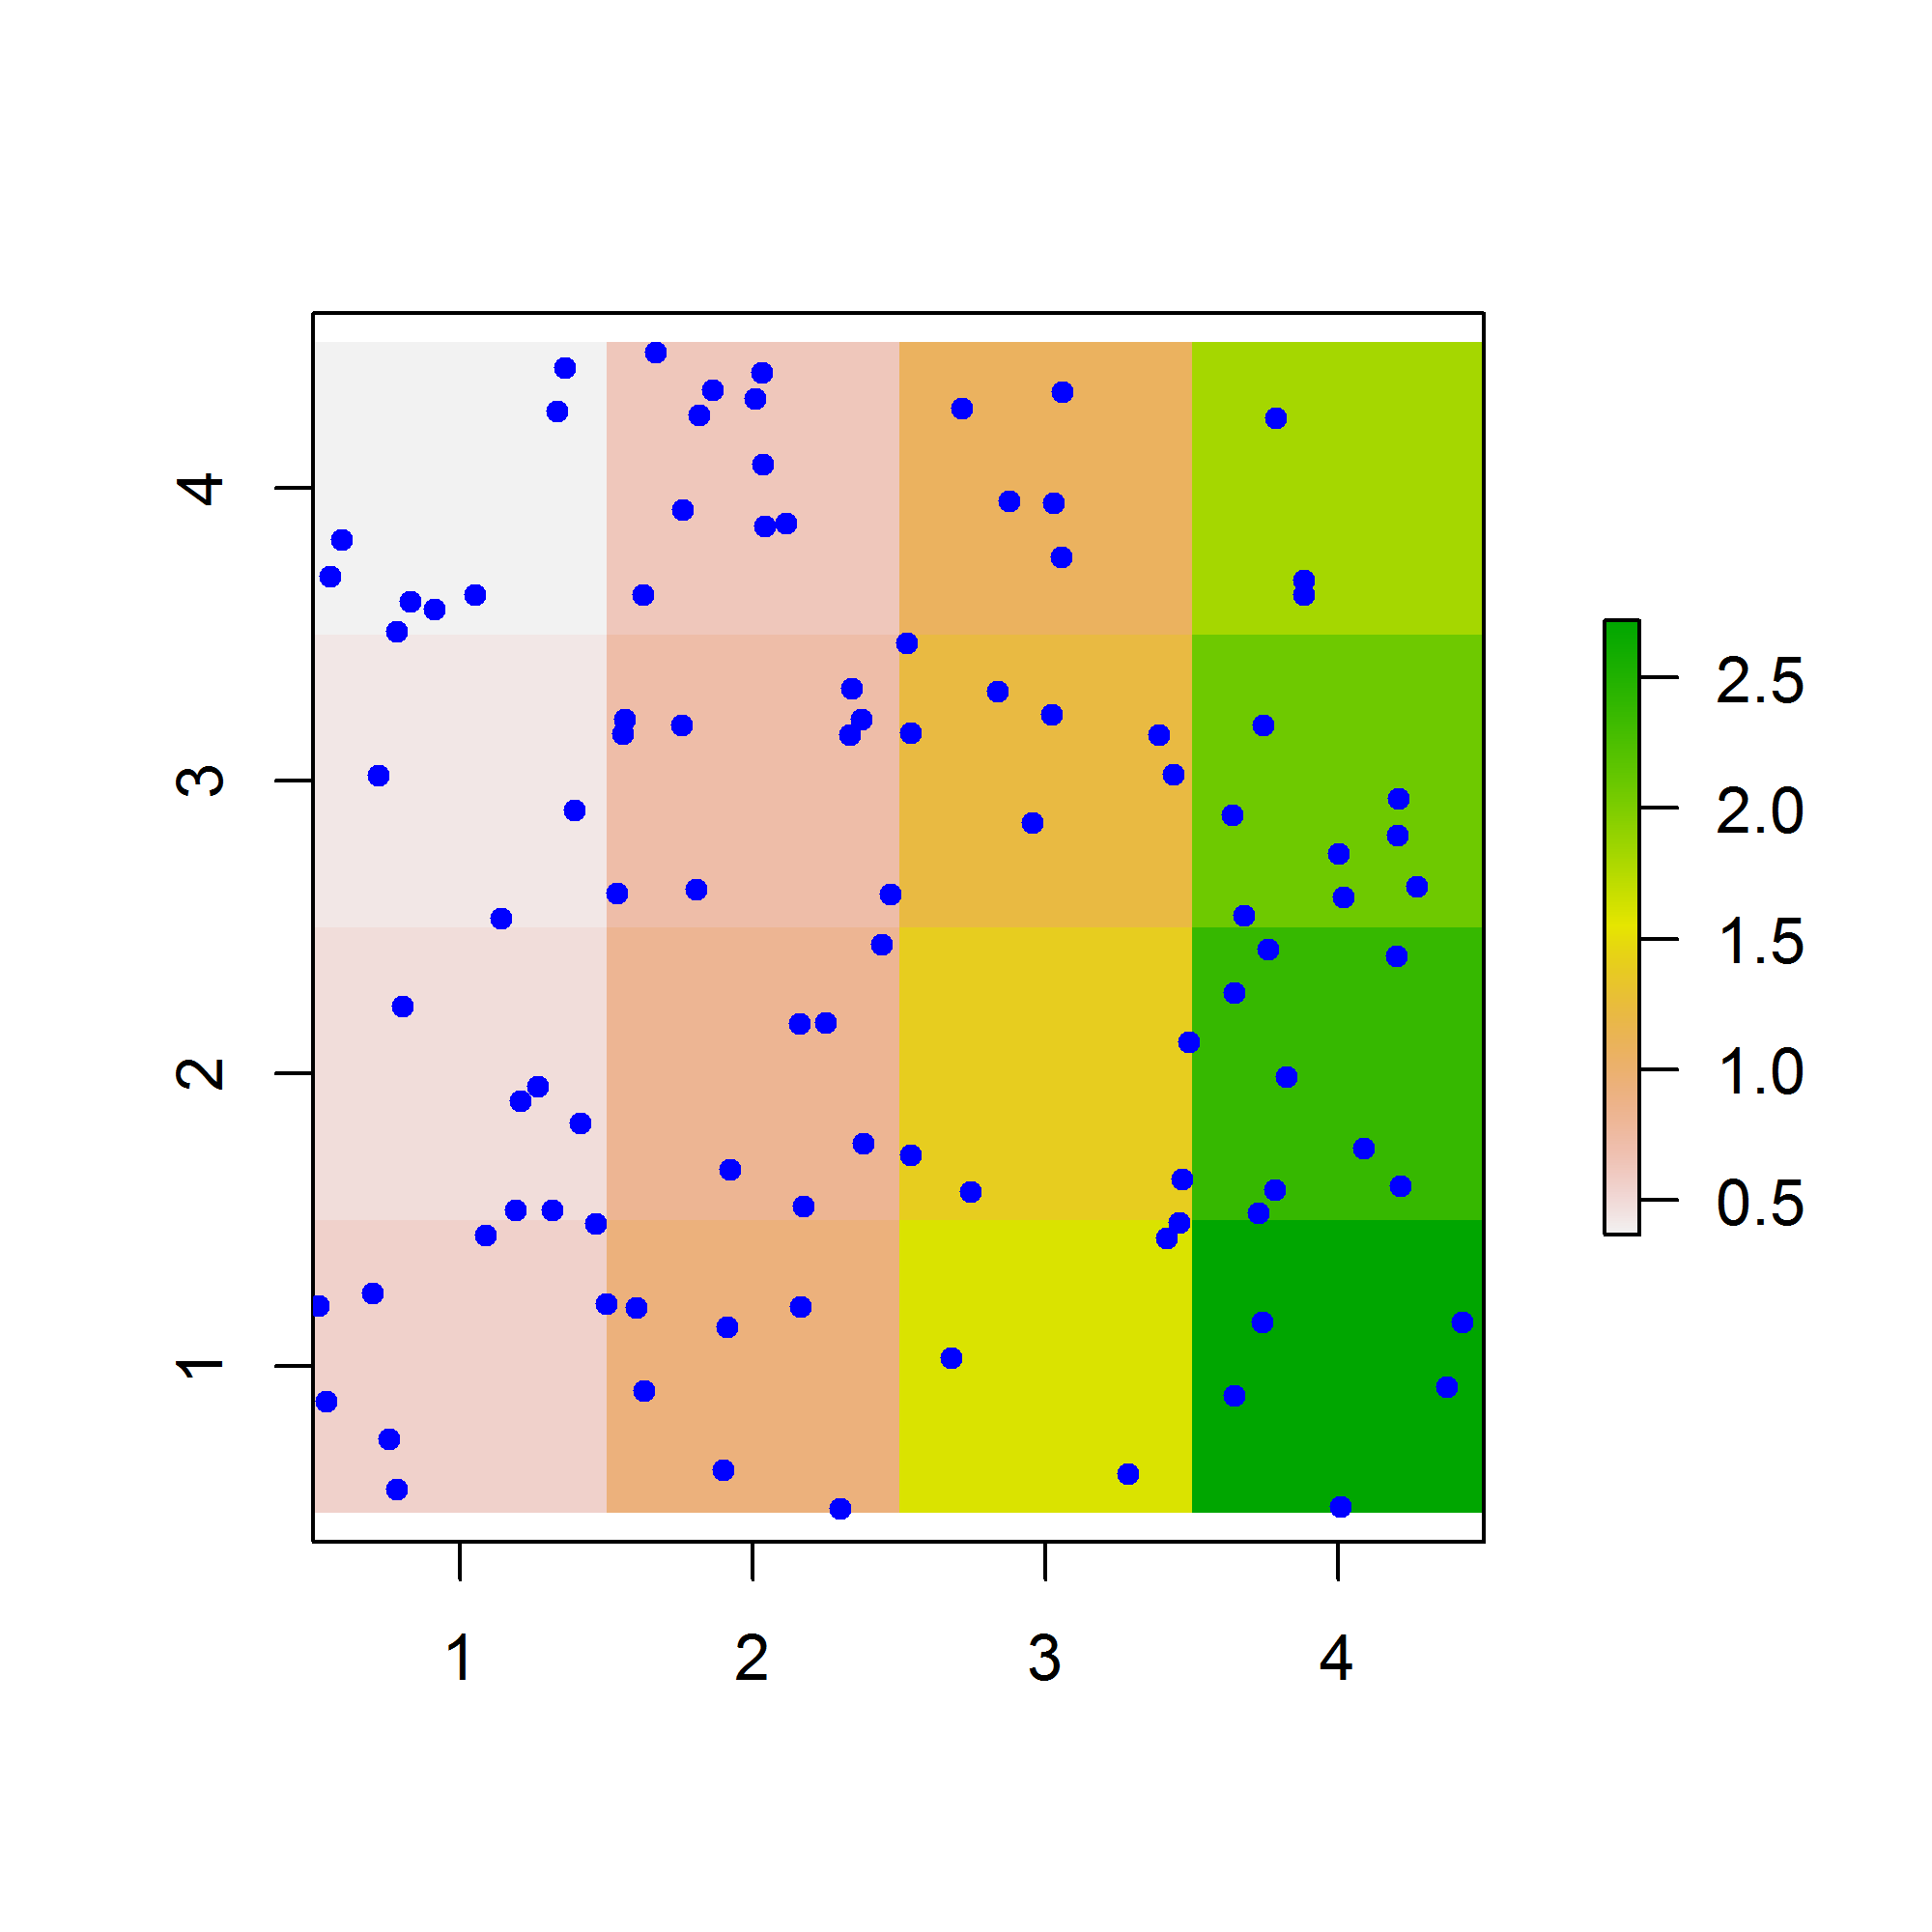
\includegraphics[height=3.25in,width=3.25in]{figs/raster_withN100}
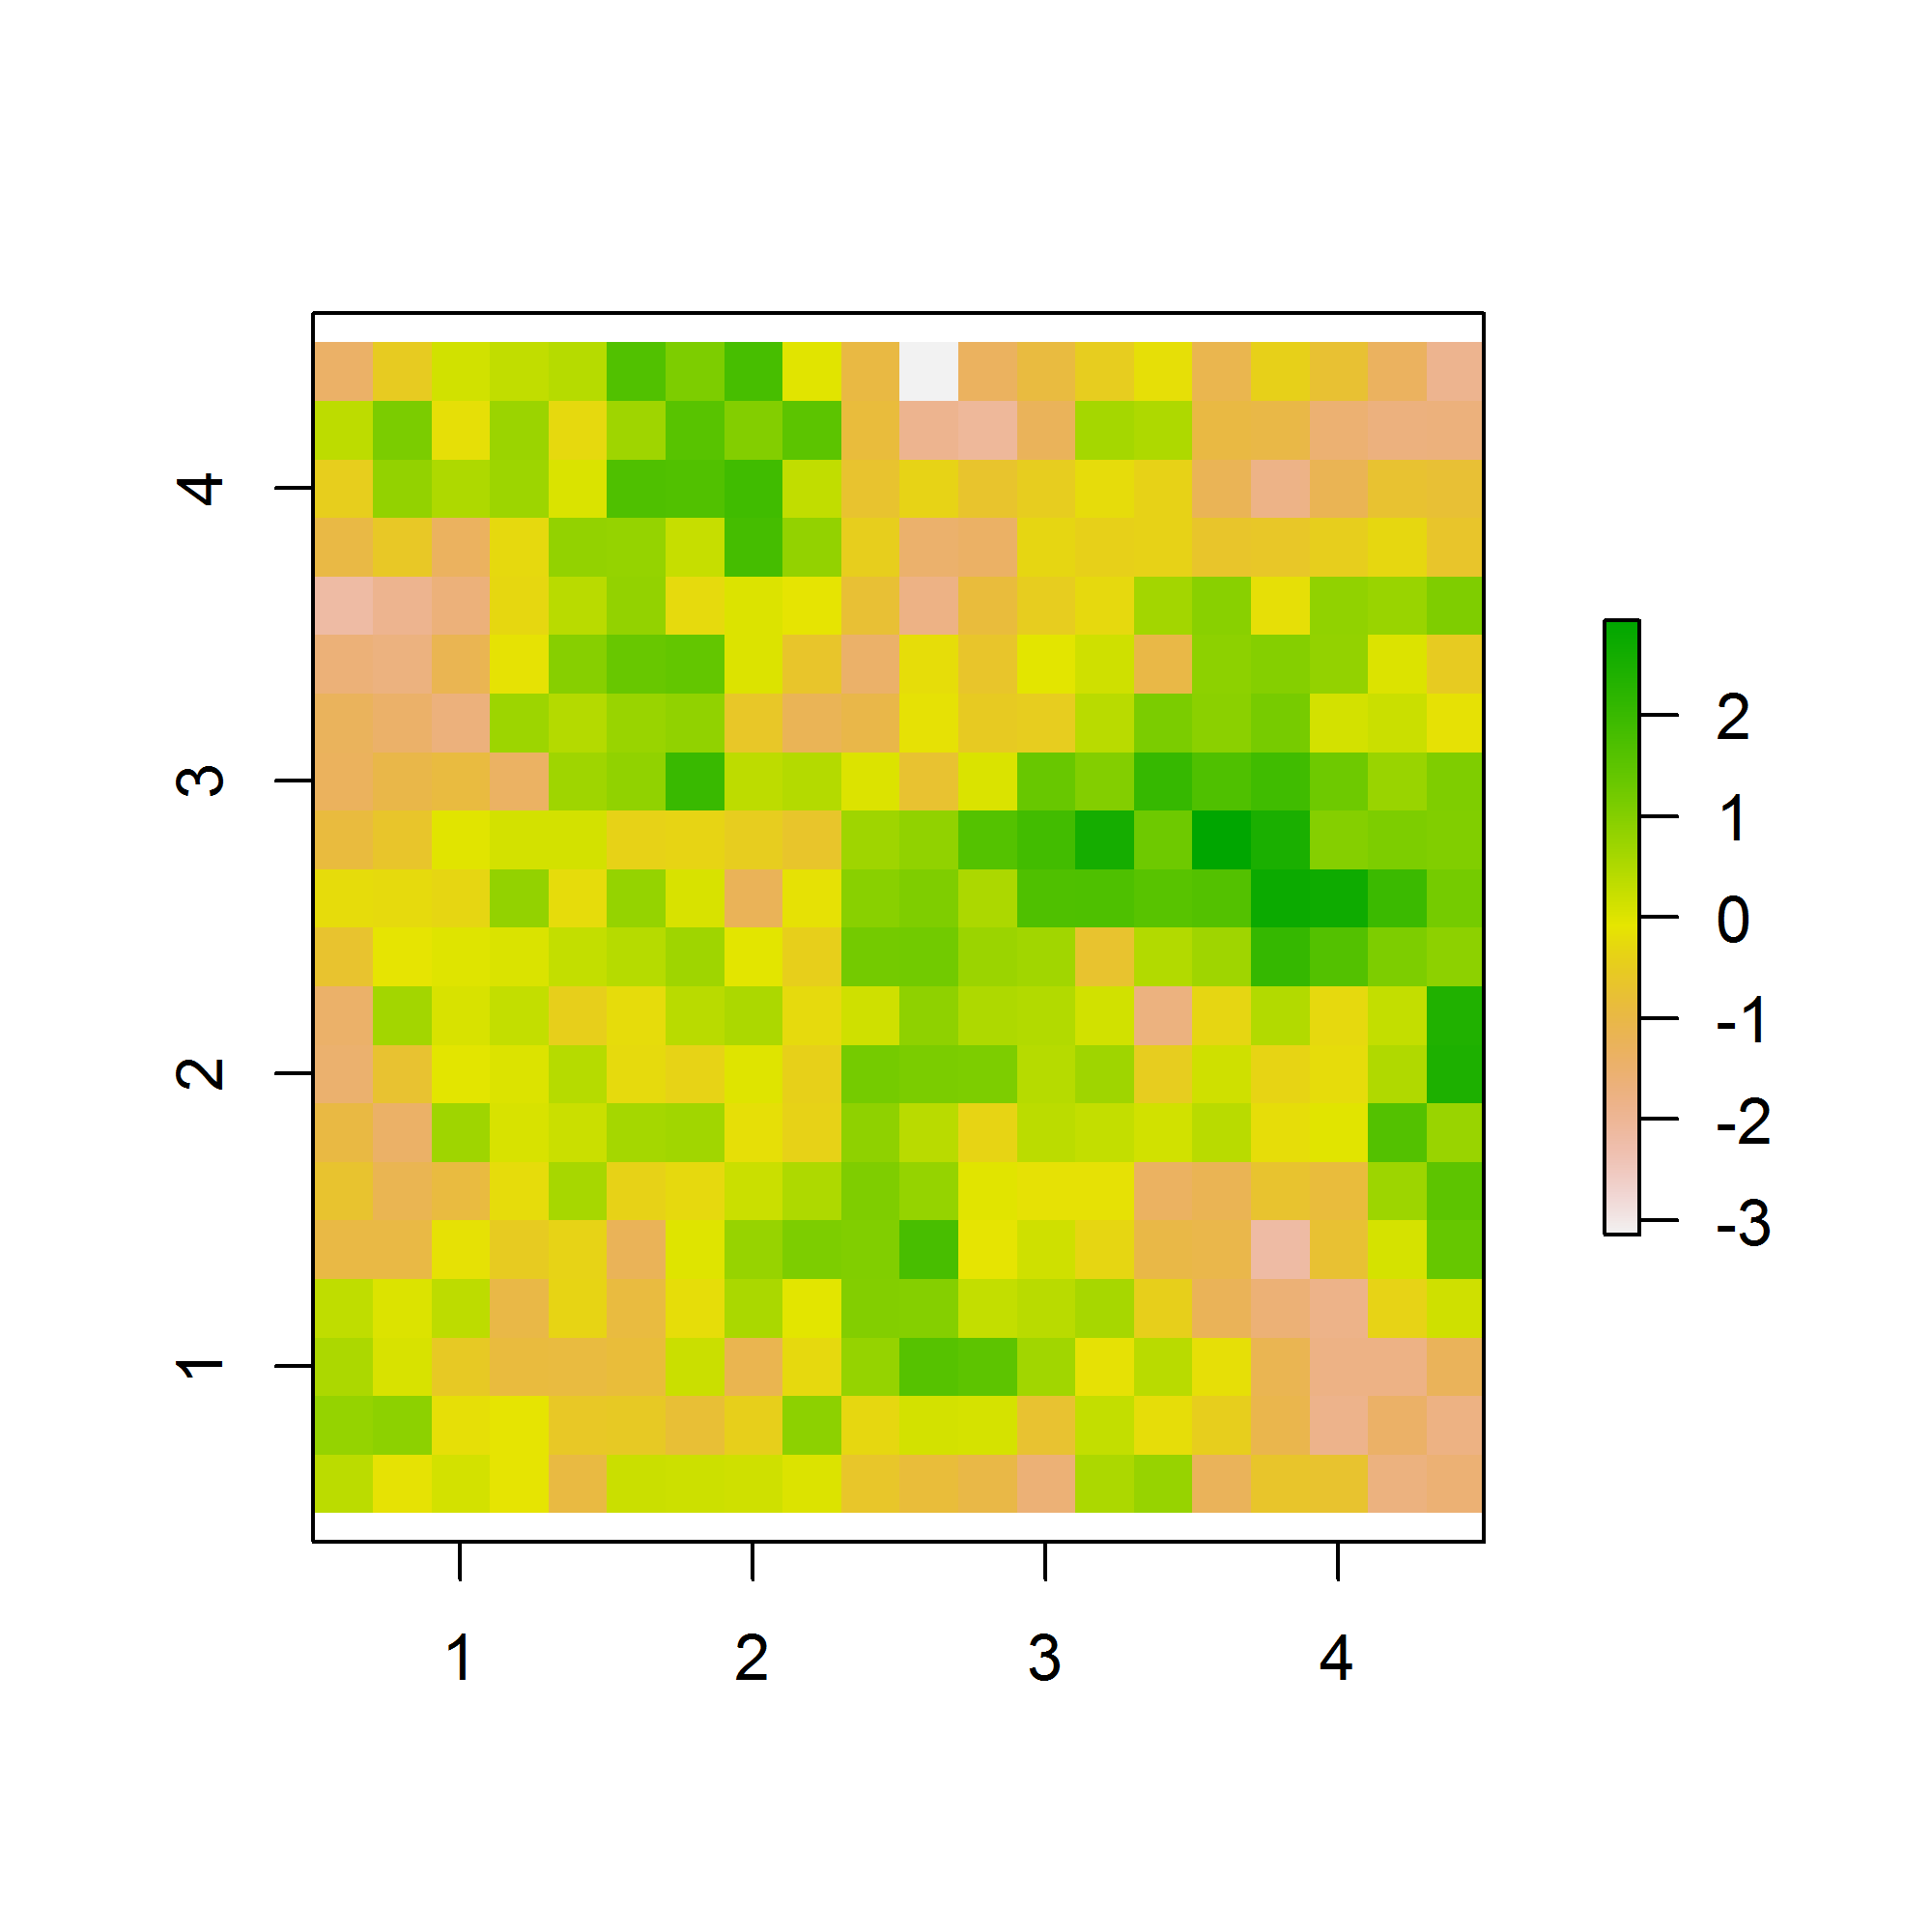
\includegraphics[height=3.25in,width=3.25in]{figs/raster_krige} &
\end{tabular}
\caption{Two covariate rasters used for simulations. A hypothetical
  realization of $N=100$ activity centers is superimposed on the left,
along with 16 trap locations. }
\label{ecoldist.fig.raster100}
\end{figure}
 


\begin{verbatim}
20 x 20 raster with nw/se trend
Summaries of sampling distribution
              N=100    E[n] = 50.89                 N=200    E[n] = XYZ
med p       mean   SD  0.025  0.50   0.975  mean   SD  0.025  0.50   0.975
euclid     64.78  6.97 50.99  64.04  77.01 130.72 10.86 111.79 130.40 152.58
ecol/known 96.84 11.89 74.53  97.49 118.37 193.69 18.87 162.87 192.30 232.34
ecol/est   99.60 13.29 74.34 101.67 126.78 198.77 21.51 165.87 197.98 238.44


Trend raster:
20 reps only 
really low
       [,1]  [,2]  [,3]   [,4]   [,5]   [,6]  [,7]   [,8]   [,9]  [,10]
[1,]  65.86 13.81 49.00  62.52  93.98 124.50 18.55  92.27 124.62 162.97
[2,] 103.45 20.30 76.12 100.39 150.54 190.36 26.05 138.87 187.36 224.37
[3,] 106.38 19.85 81.94 105.43 154.59 194.48 27.07 144.65 188.44 231.31
low
       [,1]  [,2]  [,3]   [,4]   [,5]   [,6]  [,7]   [,8]   [,9]  [,10]
[1,]  65.06  8.54 54.80  62.56  82.30 133.60 12.30 115.55 130.64 159.30
[2,]  98.11 13.94 81.99  93.43 129.75 196.62 18.19 167.41 194.49 234.94
[3,] 100.97 13.93 82.89 101.49 130.02 201.45 18.94 171.61 201.62 235.54
high
      [,1] [,2]  [,3]  [,4]   [,5]   [,6]  [,7]   [,8]   [,9]  [,10]
[1,] 68.33 5.72 59.58 69.08  79.06 141.72  7.65 129.82 141.88 154.11
[2,] 93.68 7.89 82.44 94.67 108.02 193.08 11.56 174.04 194.13 213.70
[3,] 96.86 7.96 84.58 98.96 109.30 196.53 10.89 179.08 196.45 210.77


Kriging raster: 

Really low p
       [,1]  [,2]  [,3]   [,4]   [,5]   [,6]  [,7]   [,8]   [,9]  [,10]
[1,]  75.80 15.62 49.40  78.38 101.53 161.06 43.39 110.25 154.61 253.50
[2,] 105.22 21.98 68.21 107.55 139.46 212.66 57.62 155.45 196.13 338.38
[3,] 108.67 24.48 70.40 111.43 151.81 213.13 59.30 152.83 198.22 345.64
low p
[1,]  76.08 10.28 62.80  73.23  96.85 156.73 18.01 131.87 151.79 186.19
[2,] 101.31 12.06 84.31  98.44 125.58 204.54 22.73 171.94 204.87 242.99
[3,] 102.84 11.46 88.21 100.81 124.81 203.19 22.66 171.51 199.94 242.36
> 

\end{verbatim}


\section{Discussion}

Interest in SCR models has grown rapidly in the last several years
since their formalization using likelihood \citep{borchers_efford:2008}
and Bayesian \citep{royle_young:2008} inference methods. This is because
of both the severe practical limitations of classical non-spatial
capture-recapture models, and also the ubiquity of auxiliary spatial
information in all capture-recapture studies, and thus the universal
applicability of SCR models.

All applications of SCR models have been based on models for the
encounter probability that are functions of
the standard Euclidean distance between
individuals and traps. The obvious limitations are that it is
unaffected by landscape or habitat structure and implies
stationary,  isotropic and symmetrical home ranges. These are standard
criticisms of the basic SCR model as universally applied in practice. 
In this paper,  we have developed for the first time a formal framework 
for integrating
``ecological distance'' into SCR models, where ecological distance is
defined as a cost-weighted distance between points, and where ``cost''
is characterized by one or more spatially explicit covariates that are
believe to influence movement or space-usage of individuals.  

How animals use space and therefore how distance to a trap is
perceived by individuals is not something that can ever be known. We
can only ever conjure up models to describe this
phenomenon and fit those models to limited data on a sample of individuals
during a limited amount of time. 
Historically investigators have come up with extremely simple 
models and regarded those as invariant to 
the underlying landscape. Here we have shown that there is hope to
estimate parameters, from capture-recapture data,
 that describe how animals use space and thereby
allow for irregular home range geometry that is influenced by
landscape structure.

Not surprisingly, our simulation study demonstrated that the MLE of model
parameters is approximately unbiased in moderate sample
sizes. Moreover, the 
effect of ignoring ecological distance and using normal Euclidean
distance in the model for encounter probability, has the 
logical effect of causing negative bias
in estimates of $N$. In our limited analysis the negative bias was 
severe enough so as to render the misspecified model nearly useless in
practical situations. We expect this because the effect is similar to
failing to model heterogeneity. i.e., if we misspecify ``model Mh'' with
``Model M0'' then we will expect to under-estimate $N$. So the effect of
mis-specifiying the ecological distance metric with a standard
homogeneous euclidean distance has the same effect. As a practical matter,
it stands to reason that all previous applications of SCR models based
on homogeneous distance metrics have under-stated density of the focal
population. 

In our view, this bias is not really the most important reason to consider models of
ecological distance. Rather, inference about the structure of
ecological distance is fundamental to many problems in applied and
theoretical ecology related to modeling landscape
connectivity, corridor and reserve design, population viability
analysis, gene flow, and other phenomena. 
Our new model 
allows investigators to  evaluate landscape
factors that influence movement of individuals over the landscape and
therefore SCR models based on ecological distance metrics might aid in
corridor design and understanding other aspects of space usage and
movement in animal populations. 

We adopted a standard approach to inference under our model based on
marginal likelihood \citep{borchers_efford:2008}. In principle, 
Bayesian analysis does not pose any unique challenges for this new
class of models, except that computing the cost-weighted distance is
computationally intensive. 
 So, having to do this at each iteration of an
MCMC algorithm may be impractical using existing algorithms.
A related issue is that the size of the raster slows things down. For
very large rasters, even likelihood analysis can be computationally 
challenging and methods for efficient calculation of the ecological distance
given the raster covariate(s) and parameters might be needed.
Some additional extensions of the model may be of general
interest. Instead of 
having explicit covariates it might be possible to estimate the 
``resistance surface'' as a latent field, much as \citep{wikle:2003}
 did in the developing of models of species spread based on a
 diffusion process. He defined the spatially-explicit rate of 
diffusion, $\delta(x)$, as a Gaussian spatial process and it was
estimated from the data.  The coolness of this would defy experience. 













%\end{spacing}

\newpage


\bibliography{../AndyRefs_alphabetized}
\newpage

%%\bibliography{EDmanuscript}
% Tables



% Figures








\end{document}




 

